% IEEE conference paper (IEEEtran). Compile with pdflatex (Overleaf: upload this file + figures/).
\documentclass[conference]{IEEEtran}
\usepackage{cite}
\usepackage{amsmath,amssymb}
\usepackage{graphicx}
\usepackage{booktabs}
\usepackage{url}
\usepackage{textcomp}
\usepackage{xcolor}
\usepackage{balance}
\usepackage{tikz}
\usetikzlibrary{arrows.meta,fit,backgrounds}
\newcommand{\todo}[1]{\textcolor{red}{[TODO: #1]}}
\makeatletter
\newcommand{\linebreakand}{%
  \end{@IEEEauthorhalign}
  \hfill\mbox{}\par
  \mbox{}\hfill\begin{@IEEEauthorhalign}
}
\makeatother
\begin{document}

\title{An Explainable, Auditable Real-Time Microservice for URL and QR-Code Phishing Detection: Architecture and Cross-Source Evaluation}

\author{
\IEEEauthorblockN{Advay Ravindra}
\IEEEauthorblockA{\textit{School of Computer Science and Engineering (SCOPE)} \\
\textit{Vellore Institute of Technology, Vellore}\\
\textit{advay.ravindra2023@vitstudent.ac.in}}
\and
\IEEEauthorblockN{Rishit Agrawal}
\IEEEauthorblockA{\textit{School of Computer Science and Engineering (SCOPE)} \\
\textit{Vellore Institute of Technology, Vellore}\\
\textit{rishit.agrawal2023@vitstudent.ac.in}}
\linebreakand
\IEEEauthorblockN{Dr. Naveen Kumar S.}
\IEEEauthorblockA{\textit{School of Computer Science and Engineering (SCOPE)} \\
\textit{Vellore Institute of Technology, Vellore}\\
\textit{naveenkumar.s@vit.ac.in}}
}

\maketitle

\begin{abstract}
Phishing increasingly arrives through QR codes (``quishing''), which hide the destination from conventional filters, yet most published detectors are offline classifiers that give a bare verdict, leave no audit trail and cannot act on live traffic. We present a containerised, real-time microservice that classifies both URLs and QR-code images through a single calibrated Random Forest over 35 host-level lexical features, so no page is fetched and no external threat feed is needed. Every verdict can carry SHAP feature attributions, every decision is written to separate URL and QR logs with aggregate metrics behind JWT-protected admin access, and a forward proxy can enforce verdicts on browser traffic. The service answers URL checks in 161\,ms (median) and proxy blocking decisions in 144\,ms on one worker; explanations add about 1.2\,s. We also evaluate the system itself. The QR stage tolerates blur up to $\sigma{=}2$, 0.35$\times$ downscaling, all tested rotations, JPEG compression and contrast loss, and the verdict never changes when decoding succeeds. A cross-source audit on 34{,}899 QR-derived URLs shows that benchmark accuracy overstates real performance: in both corpora the prefix \texttt{https://www.} marks every benign URL, and removing it drops the deployed model to chance (AUC 0.50) on QR URLs. We report this as a limitation and a caution for evaluating lexical detectors.
\end{abstract}

\begin{IEEEkeywords}
phishing detection, quishing, QR codes, explainable AI, SHAP, microservice, audit logging, real-time detection
\end{IEEEkeywords}

\section{Introduction}
Phishing remains one of the most common routes to credential theft and fraud: an attacker impersonates a trusted entity, usually through a link that closely resembles a legitimate address, and tricks the victim into revealing passwords or payment details \cite{zieni,li,kulkarni}. Attackers also adapt their delivery channels. QR codes are a recent example: the malicious address is embedded in an image, so text-based mail and web filters never see it, and the code is scanned by a phone outside the corporate network, a threat now called \emph{quishing} \cite{hwang,charan}. Traditional defences such as blocklists and browser warnings are reactive and struggle with the short lifetime of phishing sites, while machine-learning detectors often act as black boxes that return a verdict without a justification, limiting both user trust and an analyst's ability to review the model.

Most published detectors are offline prototypes evaluated on a fixed dataset. Few are packaged as a service that other tools can call, explain their decisions to a human, and leave an auditable trail of what was checked; fewer still handle QR images and URLs through one decision path or act on live browsing traffic. This paper presents such a system and evaluates it as a system, not only as a model.

The classifier is deliberately lightweight: it needs only the URL string, so a check involves no page download and no contact with attacker-controlled hosts, and it completes in about 160\,ms on commodity hardware. Our contributions are:
\begin{itemize}
\item A \textbf{real-time microservice} that detects phishing in URLs and QR-code images through one model, one API and one explanation format, with features recomputed from the raw URL at both training and serving time to avoid train/serve skew.
\item \textbf{Per-decision explainability}: optional SHAP attributions returned by the API and rendered in plain language, switched off on the latency-sensitive proxy path.
\item An \textbf{audit logging and metrics pipeline} with separate URL and QR histories, aggregate detection metrics and JWT-protected admin access.
\item \textbf{Network-edge enforcement}: a forward proxy that blocks flagged URLs, treats HTTP and HTTPS differently, and fails open if the service is down.
\item A deployment-oriented \textbf{evaluation}: latency, QR-decoding robustness, and a cross-source audit that exposes a benchmark shortcut inflating reported accuracy.
\end{itemize}

\section{Related Work and Research Gaps}
\textbf{Phishing detection landscape.} Zieni \textit{et al.} group detection methods into list-based, similarity-based and machine-learning approaches \cite{zieni}; Li \textit{et al.} add graph models, large language models and phishing-kit fingerprints \cite{li}; Kulkarni \textit{et al.} organise the field by the signal used: the URL string, page HTML, third-party data such as WHOIS and DNS, and page screenshots \cite{kulkarni}. Methods that fetch the live page or query third parties tend to be more accurate in the laboratory but are slower, expose the user's destination, and fail once the phishing site is offline. Deep character-level models can score very highly \cite{catal,kritika} but need more compute and are harder to explain, so classical models over hand-made URL features remain attractive for a small, fast service.

\textbf{Lexical features and tree ensembles.} A lexical feature is computed from the URL text alone (length, dot count, IP-as-host, hyphens, shorteners). Gupta \textit{et al.} showed that nine lexical features with a Random Forest can work in a real-time setting \cite{gupta}. Later studies repeatedly find tree ensembles among the strongest classical models and URL length and subdomain count among the most important features \cite{calzarossa,kustiawan,bishtawi,prakongsin}. The recurring caveat is concept drift, as attackers change how URLs look.

\textbf{Datasets.} PhiUSIIL \cite{phiusiil} provides 235{,}795 labelled URLs (134{,}850 legitimate, 100{,}945 phishing) with 54 features derived from the URL and the downloaded page, and is now a common benchmark. Many mixed-feature studies depend on page-based columns that cannot be rebuilt from the URL alone at serving time.

\textbf{Explainable detection.} SHAP and LIME are increasingly attached to phishing classifiers \cite{pavani,e2phish,poddar,armoush,kehkashan}; these works show that SHAP is applicable to phishing features, but they typically stop at plots in a notebook.

\textbf{Quishing.} Quishing research is newer. Kim and Hwang couple an AutoML URL classifier with a QR reader \cite{hwang}; Charan and Thilak treat fake payment QR codes and links together \cite{charan}; Ford and Berry use a CNN to locate QR codes in email images \cite{ford}. Two 2025 studies compare classifying the QR \emph{image} directly with decoding it and classifying the URL \cite{trad,cyberai}. We follow the decode-then-classify route, so one lexical model serves both inputs.

\textbf{Research gaps.} Across these works we identify six gaps that this project addresses:
\begin{enumerate}
\item \textbf{Detection stops at a model:} few works provide a service that accepts live input, writes an audit record and lets an administrator review it later.
\item \textbf{Features unavailable at serving time:} HTML, WHOIS or traffic features help offline but slow requests and leak destinations.
\item \textbf{Train/serve mismatch:} features precomputed in a public CSV may differ from what a live extractor produces; this is rarely treated as a design problem.
\item \textbf{Explanations stay in notebooks:} few systems expose an optional explanation on a live API or skip it where latency matters.
\item \textbf{Quishing treated separately:} little work uses one lexical model for typed and decoded URLs, or records an ``unreadable QR'' outcome instead of forcing a label.
\item \textbf{No live enforcement path:} forward-proxy blocking that calls the same detection API, fails open and handles HTTP and HTTPS differently is rarely shipped.
\end{enumerate}

\section{System Architecture}
Three Docker Compose services cooperate (Fig.~\ref{fig:arch}): a FastAPI inference service, a React single-page frontend served by nginx, and a forward proxy. All clients call the same REST API, so the web interface, the proxy and any future client reuse identical detection logic. The prediction endpoints are open, whereas logs and metrics require an administrator token.

\begin{figure*}[t]
\centering
\resizebox{\textwidth}{!}{%
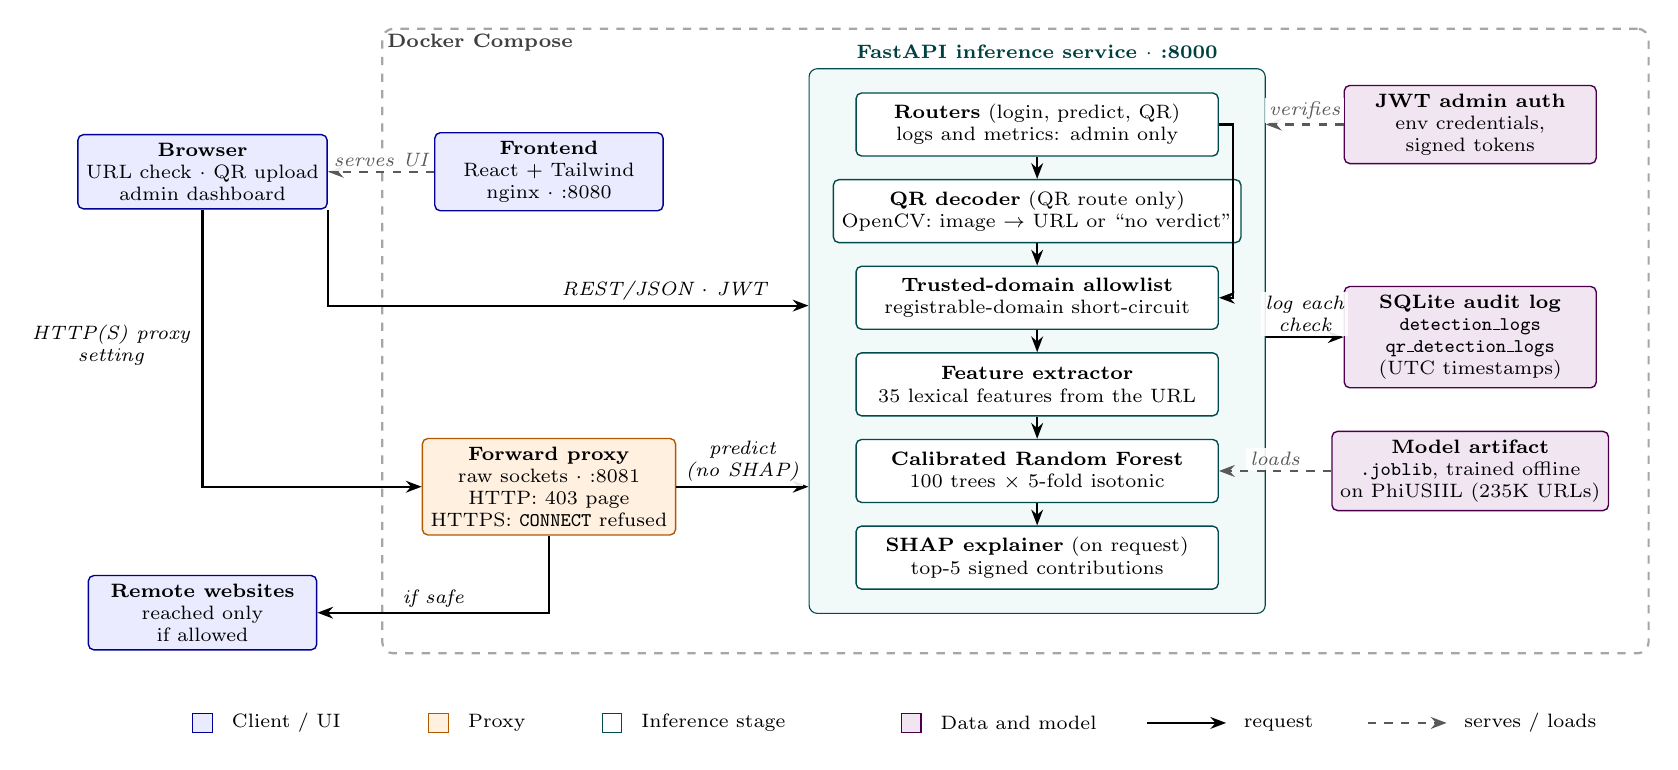
\begin{tikzpicture}[font=\scriptsize,
  box/.style={draw, rounded corners=2pt, align=center, inner sep=3pt, minimum height=8mm, line width=0.5pt},
  client/.style={box, fill=blue!8, draw=blue!60!black, minimum width=29mm},
  proxybox/.style={box, fill=orange!12, draw=orange!70!black, minimum width=32mm},
  stage/.style={box, fill=white, draw=teal!60!black, minimum width=46mm},
  store/.style={box, fill=violet!10, draw=violet!60!black, minimum width=32mm},
  flow/.style={-{Stealth[length=2mm]}, thick},
  aux/.style={-{Stealth[length=2mm]}, thick, dashed, gray!70!black},
  lab/.style={font=\scriptsize\itshape, align=center, inner sep=1.5pt, fill=white, fill opacity=0.9, text opacity=1}]

% ---------- clients and edge services ----------
\node[client] (browser) at (0,2.4) {\textbf{Browser}\\URL check $\cdot$ QR upload\\admin dashboard};
\node[client] (frontend) at (4.4,2.4) {\textbf{Frontend}\\React + Tailwind\\nginx $\cdot$ :8080};
\node[proxybox] (proxy) at (4.4,-1.6) {\textbf{Forward proxy}\\raw sockets $\cdot$ :8081\\HTTP: 403 page\\HTTPS: \texttt{CONNECT} refused};
\node[client] (remote) at (0,-3.2) {\textbf{Remote websites}\\reached only\\if allowed};

% ---------- inference service pipeline ----------
\node[stage] (n1) at (10.6,3.0) {\textbf{Routers} (login, predict, QR)\\logs and metrics: admin only};
\node[stage] (n2) at (10.6,1.9) {\textbf{QR decoder} (QR route only)\\OpenCV: image $\rightarrow$ URL or ``no verdict''};
\node[stage] (n3) at (10.6,0.8) {\textbf{Trusted-domain allowlist}\\registrable-domain short-circuit};
\node[stage] (n4) at (10.6,-0.3) {\textbf{Feature extractor}\\35 lexical features from the URL};
\node[stage] (n5) at (10.6,-1.4) {\textbf{Calibrated Random Forest}\\100 trees $\times$ 5-fold isotonic};
\node[stage] (n6) at (10.6,-2.5) {\textbf{SHAP explainer} (on request)\\top-5 signed contributions};

% ---------- data and model ----------
\node[store] (jwt) at (16.1,3.0) {\textbf{JWT admin auth}\\env credentials,\\signed tokens};
\node[store] (sqlite) at (16.1,0.3) {\textbf{SQLite audit log}\\\texttt{detection\_logs}\\\texttt{qr\_detection\_logs}\\(UTC timestamps)};
\node[store] (model) at (16.1,-1.4) {\textbf{Model artifact}\\\texttt{.joblib}, trained offline\\on PhiUSIIL (235K URLs)};

% ---------- containers (drawn behind the nodes) ----------
\begin{scope}[on background layer]
  \node[draw=teal!60!black, rounded corners=3pt, fill=teal!5, inner sep=3mm,
        fit=(n1)(n2)(n3)(n4)(n5)(n6),
        label={[font=\scriptsize\bfseries, text=teal!50!black]above:FastAPI inference service $\cdot$ :8000}] (api) {};
  \node[draw=gray!70, dashed, thick, rounded corners=4pt, inner sep=5mm,
        fit=(frontend)(proxy)(api)(jwt)(sqlite)(model),
        label={[font=\scriptsize\bfseries, anchor=north west, inner sep=2pt, text=gray!50!black]north west:Docker Compose}] (docker) {};
\end{scope}

% ---------- request flow ----------
\draw[aux]  (frontend.west) -- node[lab, above] {serves UI} (browser.east);
\draw[flow] (browser.south east) |- node[lab, pos=0.85, above] {REST/JSON $\cdot$ JWT} ([yshift=0.45cm]api.west);
\draw[flow] (browser.south) |- (proxy.west);
\node[lab, anchor=east] at (-0.1,0.2) {HTTP(S) proxy\\setting};
\draw[flow] (proxy.east) -- node[lab, above] {predict\\(no SHAP)} (api.west |- proxy.east);
\draw[flow] (proxy.south) |- node[lab, pos=0.75, above] {if safe} (remote.east);

% ---------- inside the service ----------
\draw[flow] (n1.south) -- (n2.north);
\draw[flow] (n2.south) -- (n3.north);
\draw[flow] (n3.south) -- (n4.north);
\draw[flow] (n4.south) -- (n5.north);
\draw[flow] (n5.south) -- (n6.north);
\draw[flow] (n1.east) -- ++(0.18,0) |- (n3.east);   % URL route skips the QR decoder

% ---------- data and model links ----------
\draw[aux]  (jwt.west) -- node[lab, above] {verifies} (jwt.west -| api.east);
\draw[flow] (sqlite.west -| api.east) -- node[lab, above] {log each\\check} (sqlite.west);
\draw[aux]  (model.west) -- node[lab, above] {loads} (n5.east);

% ---------- legend ----------
\node[draw=blue!60!black, fill=blue!8, minimum size=2.5mm, inner sep=0] at (0,-4.6) {};
\node[anchor=west] at (0.25,-4.6) {Client / UI};
\node[draw=orange!70!black, fill=orange!12, minimum size=2.5mm, inner sep=0] at (3.0,-4.6) {};
\node[anchor=west] at (3.25,-4.6) {Proxy};
\node[draw=teal!60!black, fill=white, minimum size=2.5mm, inner sep=0] at (5.2,-4.6) {};
\node[anchor=west] at (5.45,-4.6) {Inference stage};
\node[draw=violet!60!black, fill=violet!10, minimum size=2.5mm, inner sep=0] at (9.0,-4.6) {};
\node[anchor=west] at (9.25,-4.6) {Data and model};
\draw[flow] (12.0,-4.6) -- (13.0,-4.6);
\node[anchor=west] at (13.1,-4.6) {request};
\draw[aux] (14.8,-4.6) -- (15.8,-4.6);
\node[anchor=west] at (15.9,-4.6) {serves / loads};
\end{tikzpicture}}
\caption{Architecture of the detection microservice. The three Docker Compose services (frontend, forward proxy, inference service) share one REST API. QR images are decoded and then follow the same pipeline as typed URLs, and every decision is written to the matching log table.}
\label{fig:arch}
\end{figure*}

\subsection{URL classifier}
Thirty-five lexical features are computed from the URL host: length and count statistics, IP-as-host, subdomain depth, hyphens, suspicious and known TLDs, URL shorteners, punycode and phishing keywords. No external lookup or page fetch is needed, which keeps latency low and avoids contacting attacker-controlled hosts. The model is a 100-tree Random Forest \cite{breiman} wrapped in 5-fold isotonic calibration \cite{nm2005} so the returned confidence is a usable probability. It is trained on PhiUSIIL \cite{phiusiil} with bare-domain augmentation of \texttt{www.} URLs, and a small allowlist of high-reputation domains short-circuits to ``legitimate''. Features are always recomputed from the raw URL with the same function used at inference, which removes train/serve skew. Scope is deliberately limited to the host so that ordinary pages, such as login paths on trusted sites, are not penalised.

\subsection{QR-code pipeline}
Uploaded images (at most 5\,MB) are decoded with OpenCV's \texttt{QRCodeDetector}. The first URL in the payload is classified by the same model and explained. Unreadable images, and QR codes that contain no URL, return an explicit ``no verdict'' response instead of a guess, and are still logged.

\subsection{Explainable AI}
For each requested explanation, SHAP \cite{shap} contributions toward the phishing class are computed for each calibration fold and averaged. The response contains the five most influential features, each with a plain-language label, its value, a signed contribution and its direction (toward ``phishing'' or ``legitimate''); the frontend renders them beside the verdict. Explanations are computed on request so that callers on a latency-critical path, such as the proxy, do not pay for them. Fig.~\ref{fig:seq} traces one explained URL check from the browser to the log.

\begin{figure*}[t]
\centering
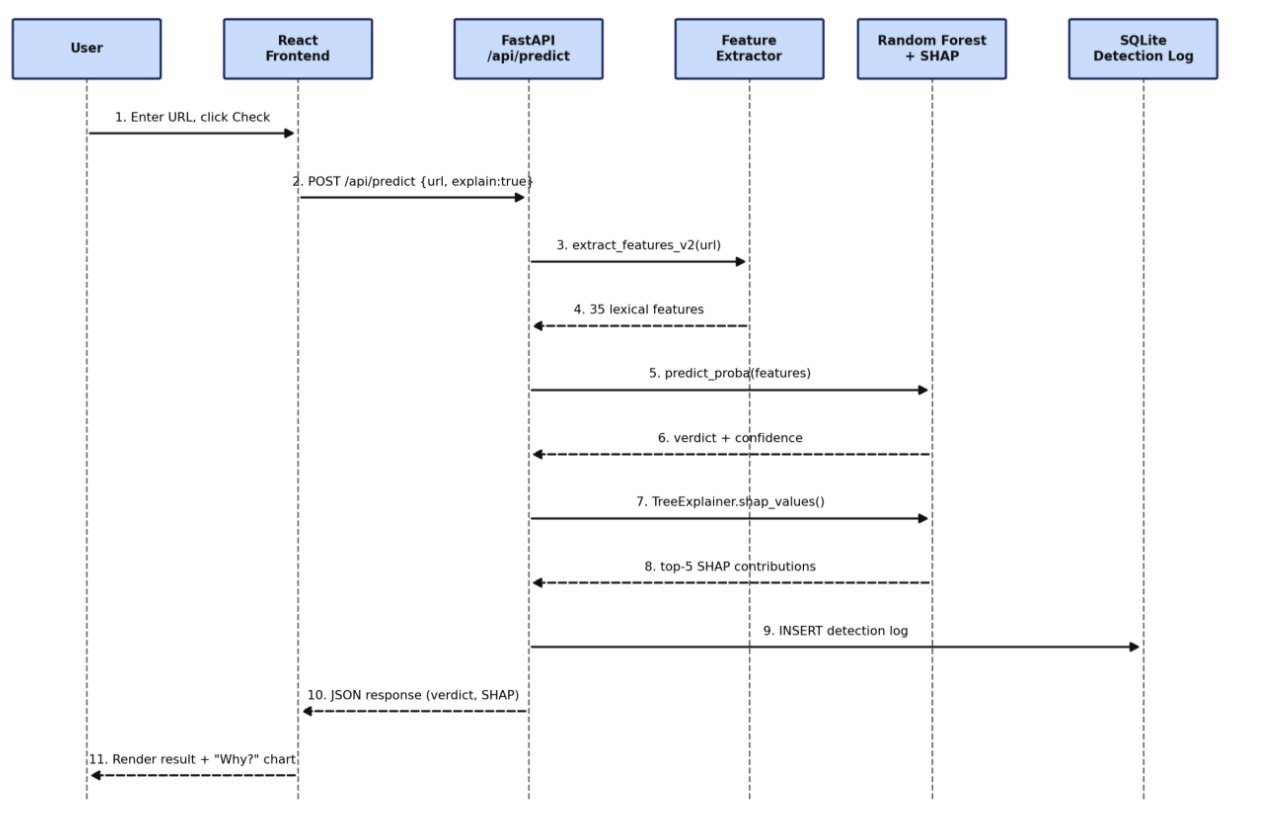
\includegraphics[width=\textwidth]{figures/sequence.jpg}
\caption{Sequence of a URL check with an explanation. Allowlisted domains return before step~3. The proxy issues the same call with \texttt{explain=false} and so skips steps~7 and~8; QR uploads add a decoding step and are written to the QR log table.}
\label{fig:seq}
\end{figure*}

\subsection{Logging and metrics pipeline}
Every decision is written to SQLite in two separate tables: URL checks (URL, verdict, confidence, message, UTC timestamp) and QR checks (filename, decoded URL, readability, verdict, confidence, message, timestamp), so QR history never mixes with URL history. Admin-only endpoints expose the most recent logs (configurable limit) and aggregate metrics: total checks, phishing detected and detection rate, plus unreadable count and readable rate for QR. Access uses a username and password login that issues a signed JWT with configurable lifetime; the dashboard and log pages consume these endpoints.

\subsection{Network-edge enforcement}
A forward proxy built on raw sockets queries the API for each request. For plain HTTP it sees the full URL and returns a custom 403 warning page for flagged URLs. For HTTPS it sees only the host in the \texttt{CONNECT} request, so flagged hosts have the tunnel refused and the browser shows its own connection error. Loopback hosts bypass checking, and if the API is unreachable the proxy fails open to avoid breaking browsing. It listens on the loopback interface only, to avoid exposing an open proxy.

\subsection{Deployment}
The three services are defined in Docker Compose; the API exposes a health endpoint used by a container health check, and the proxy starts only after the API is healthy. A GitHub Actions workflow runs on pushes and pull requests to the main branch and builds and pushes the image to a registry on pushes. Credentials are supplied through repository secrets and environment variables. The prototype targets a single host and is validated at technology readiness level 3 (proof of concept).

\section{Evaluation Setup}
\textbf{Data.} PhiUSIIL \cite{phiusiil}: 235{,}795 URLs, split 80/20 stratified (seed 42) exactly as in the training script (188{,}636 train / 47{,}159 test; 42.8\% phishing in test). QR dataset \cite{malibariqr}: 100{,}000 benign and 100{,}000 malicious QR images generated from the URLs of \cite{malibariurl}, whose malicious class includes defacement and malware URLs as well as phishing; the dataset states no licence and was used locally. A random sample of 20{,}000 per class was decoded with the production decoder (95.1\% / 94.7\% decodable), yielding 34{,}899 unique URLs (49.8\% malicious).

\textbf{Environment.} Latency was measured against an isolated instance of the production code (separate log database), with a single uvicorn worker on an Apple MacBook Air (M4, 10-core CPU, 16\,GB RAM) and the client on the same host. Times are wall-clock per HTTP request.

\section{Results}
\subsection{System performance}
Table~\ref{tab:lat} reports latency. A plain URL check has a median of 161\,ms ($p_{95}$ 169\,ms) and sustains about 20 requests/s with eight concurrent clients on one worker. Requests that include a SHAP explanation, which includes every QR check, take about 1.4\,s. The proxy's blocking decision (88 of 88 flagged HTTP URLs blocked) costs 144\,ms median, essentially one API call. Per-request cost is dominated by inference over the 500 trees of the calibrated forest, so batching, model compression or caching are the main levers for higher throughput.

\begin{table}[t]
\caption{Latency of the deployed service (single worker, ms)}
\label{tab:lat}
\centering
\small
\begin{tabular}{lcccc}
\toprule
Endpoint & $n$ & p50 & p95 & p99 \\
\midrule
URL check & 500 & 161 & 169 & 195 \\
URL check + SHAP & 100 & 1404 & 1430 & 1453 \\
URL check, 8 clients & 500 & 440 & 499 & 519 \\
QR check (decode + SHAP) & 200 & 1407 & 1447 & 1458 \\
Proxy block decision & 88 & 144 & 151 & 231 \\
\bottomrule
\end{tabular}
\\[2pt]\footnotesize URL check at 8 clients: 19.8 requests/s.
\end{table}

\subsection{QR decoding robustness}\label{sec:res-qr}
For 2{,}000 images per class we degraded each image one way at a time at four strengths and ran the production decoder and classifier. Clean decode rate is 95.4\% (benign 95.2\%, malicious 95.6\%). Whenever a degraded image still decodes, the decoded URL and the verdict equal the clean ones in 100\% of cases, so image quality affects the \emph{availability} of a verdict, not its correctness. Fig.~\ref{fig:rob} and Table~\ref{tab:rob} show that decoding fails abruptly (noise and occlusion) rather than gradually. Mild blur and downscaling raise the decode rate above the clean baseline, which suggests the detector is sensitive to crisp synthetic renders and that a light-blur retry could recover failures.

\begin{figure*}[t]
\centering
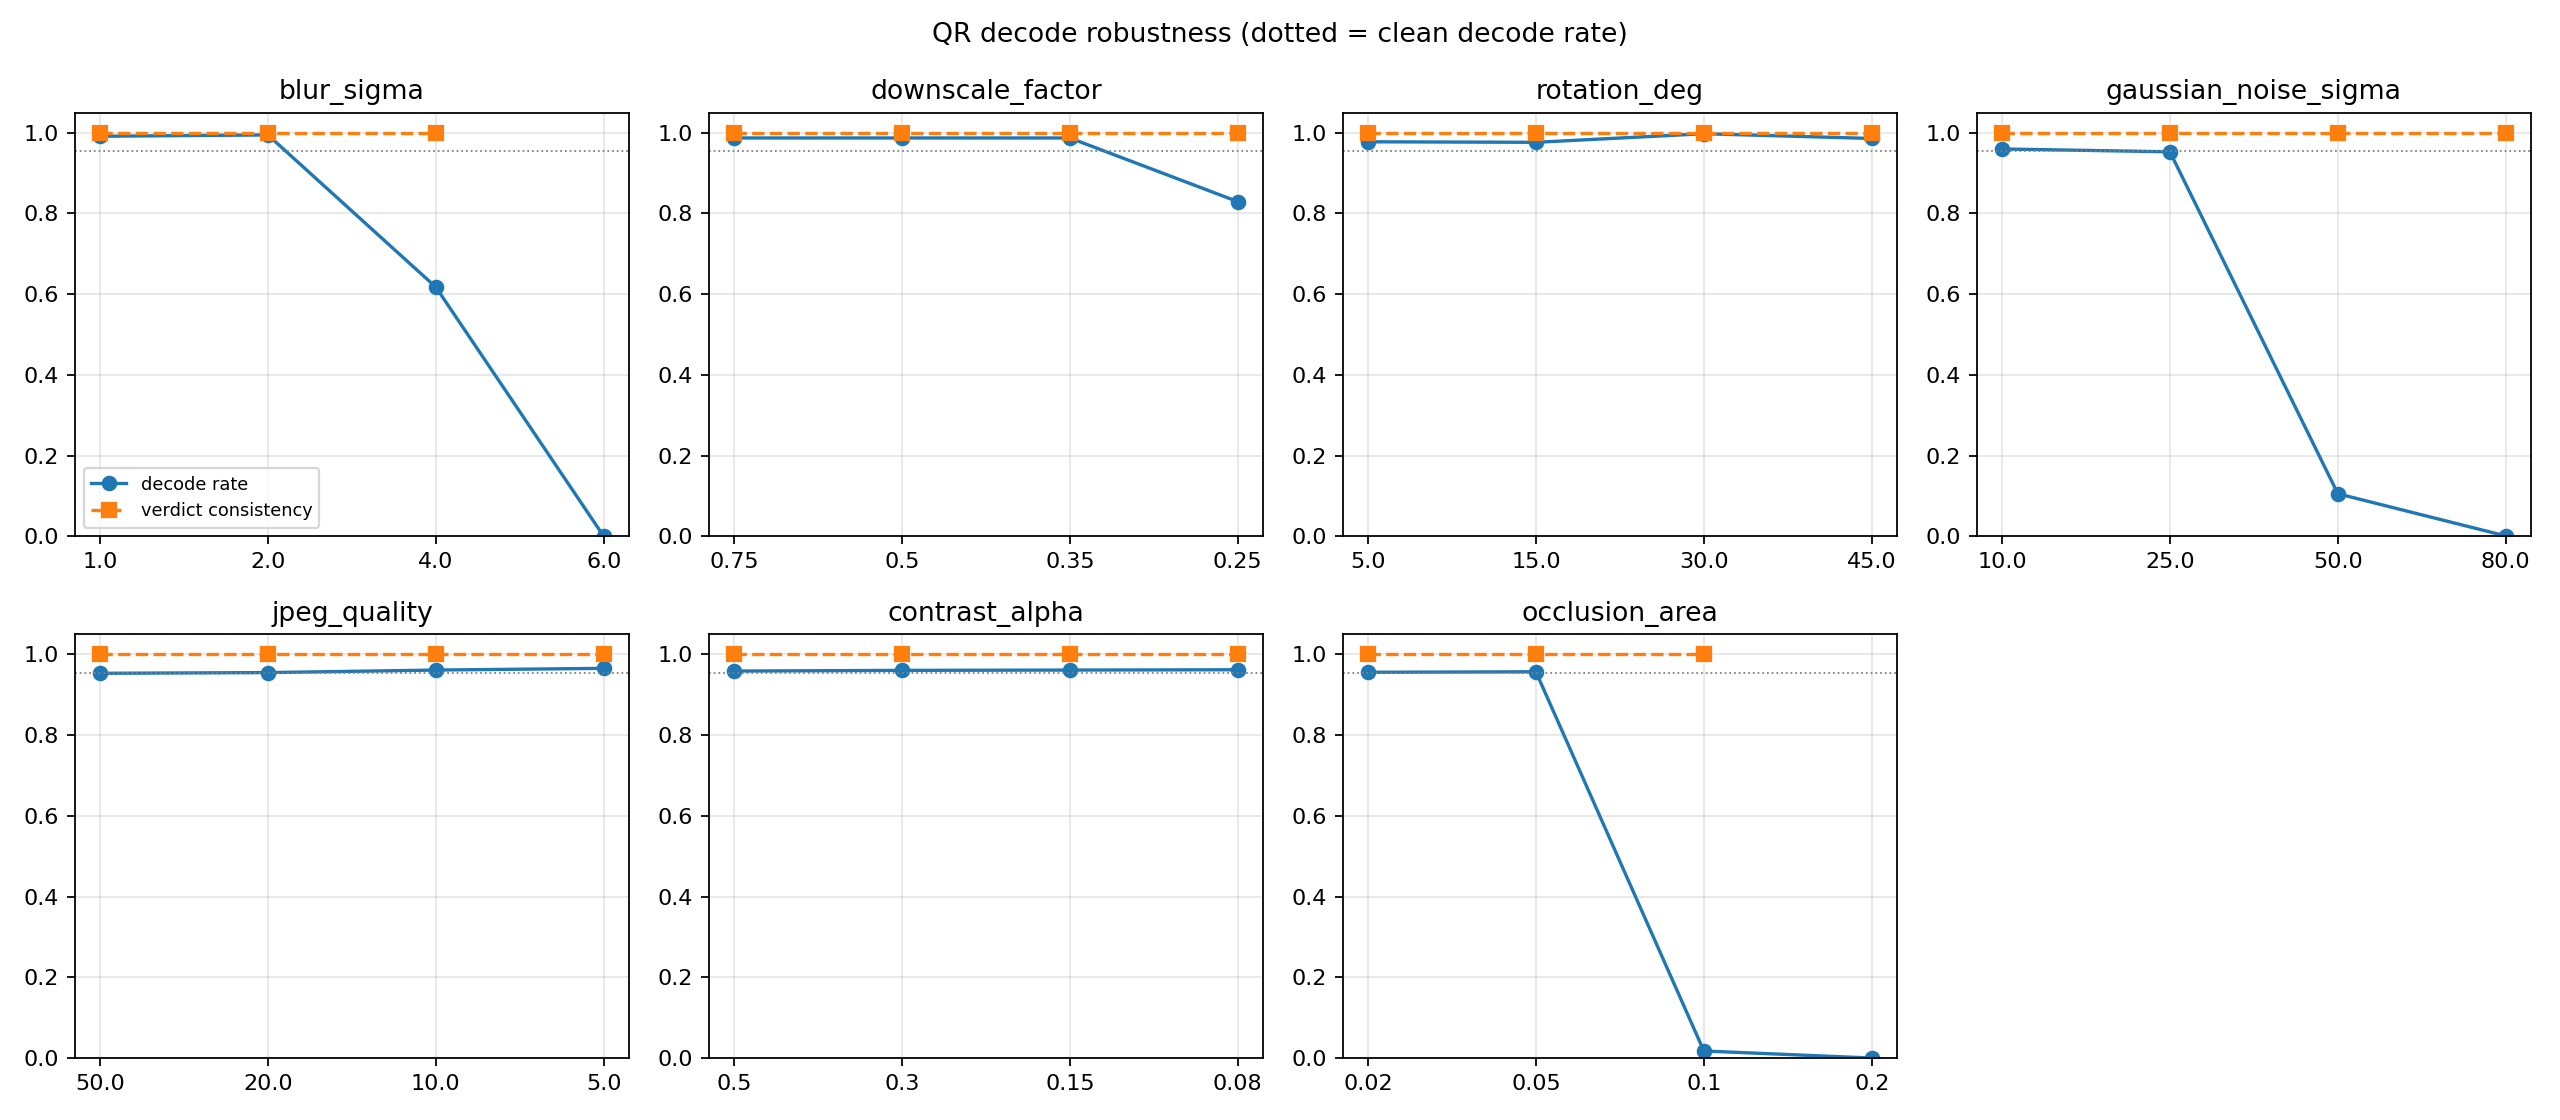
\includegraphics[width=\textwidth]{figures/qr_robustness.png}
\caption{Decode rate (circles) and verdict consistency (squares) versus degradation strength; dotted line is the clean decode rate.}
\label{fig:rob}
\end{figure*}

\begin{table}[t]
\caption{Decode rate under degradation (2{,}000 images/class; clean = 0.954)}
\label{tab:rob}
\centering
\small
\begin{tabular}{lcccc}
\toprule
Degradation & L1 & L2 & L3 & L4 \\
\midrule
Blur $\sigma$ (1,2,4,6) & .991 & .994 & .618 & .000 \\
Downscale (.75,.5,.35,.25) & .987 & .987 & .987 & .829 \\
Rotation$^\circ$ (5,15,30,45) & .978 & .976 & .998 & .986 \\
Noise $\sigma$ (10,25,50,80) & .960 & .953 & .106 & .001 \\
JPEG $q$ (50,20,10,5) & .953 & .955 & .961 & .965 \\
Contrast $\alpha$ (.5,.3,.15,.08) & .958 & .960 & .961 & .962 \\
Occlusion area (.02,.05,.10,.20) & .956 & .957 & .018 & .000 \\
\bottomrule
\end{tabular}
\end{table}

\subsection{Detection quality and cross-source generalization}
Table~\ref{tab:cur} reports the deployed model. On its own test split it is precise but conservative (precision 0.989, recall 0.647, ROC-AUC 0.881), reflecting the host-only scope. On QR-derived URLs accuracy falls to 0.555 and expected calibration error (ECE, 10 bins) rises from 0.143 to 0.380, so confidences should not be trusted across sources. The corpora differ structurally (Table~\ref{tab:prof}): 77.5\% of benign QR URLs carry a path versus 0\% in PhiUSIIL, and only 5.6\% of QR phishing URLs use HTTPS versus 49\%. Only 72 QR URLs appear verbatim in PhiUSIIL, with agreeing labels.

\begin{table}[t]
\caption{Deployed model: in-distribution vs.\ QR-derived URLs}
\label{tab:cur}
\centering
\small
\begin{tabular}{lccccc}
\toprule
Test set & Acc & Prec & Rec & AUC & ECE \\
\midrule
PhiUSIIL test & .846 & .989 & .647 & .881 & .143 \\
QR URLs & .555 & .590 & .345 & .703 & .380 \\
\bottomrule
\end{tabular}
\end{table}

\begin{table}[t]
\caption{Corpus profile (share of URLs)}
\label{tab:prof}
\centering
\small
\begin{tabular}{llcccc}
\toprule
Corpus & Class & HTTPS & \texttt{www.} & Path & IP host \\
\midrule
PhiUSIIL & benign & 1.00 & 1.00 & 0.00 & 0.00 \\
PhiUSIIL & phishing & .49 & .42 & .27 & .005 \\
QR & benign & 1.00 & 1.00 & .78 & 0.00 \\
QR & phishing & .06 & .13 & .90 & .04 \\
\bottomrule
\end{tabular}
\end{table}

\subsection{A benchmark shortcut}\label{sec:res-shortcut}
Baselines trained on the same data (logistic regression, Random Forest and gradient boosting on the same features, and a hashed character $n$-gram model on the full URL) appear to transfer well: character $n$-grams reach AUC 0.996--0.999 across sources. However, in both corpora the prefix \texttt{https://www.} marks \emph{all} benign URLs but only 2.5\% (PhiUSIIL) and 0.6\% (QR) of phishing URLs. After stripping the scheme and leading \texttt{www.} from every URL (Table~\ref{tab:base}) the deployed model scores AUC 0.501 on QR URLs, the PhiUSIIL-trained boosting model 0.494, and the character model trained on PhiUSIIL falls from 0.996 to 0.626 on QR. Character $n$-grams keep more signal within a source (QR$\rightarrow$QR 0.965), indicating that path content is informative but source-specific.

\begin{table}[t]
\caption{ROC-AUC before / after removing scheme and \texttt{www.} (train $\rightarrow$ test)}
\label{tab:base}
\centering
\small
\begin{tabular}{lcc}
\toprule
Model (train $\rightarrow$ test) & Original & Stripped \\
\midrule
Deployed RF, Phi $\rightarrow$ QR & .703 & .501 \\
HistGB (lexical), Phi $\rightarrow$ QR & .914 & .494 \\
HistGB (lexical), QR $\rightarrow$ QR & .974 & .766 \\
HistGB (lexical), QR $\rightarrow$ Phi & .780 & .672 \\
Char $n$-gram, Phi $\rightarrow$ Phi & .999 & .950 \\
Char $n$-gram, Phi $\rightarrow$ QR & .996 & .626 \\
Char $n$-gram, QR $\rightarrow$ QR & .999 & .965 \\
Char $n$-gram, QR $\rightarrow$ Phi & .995 & .797 \\
\bottomrule
\end{tabular}
\end{table}

\section{Discussion}
\textbf{System design.} The central design choice is to classify from the URL string alone. This keeps latency low, protects privacy and avoids fetching pages, at the cost of a reputation signal: recall on the benchmark is 0.647, and the host-only scope misses phishing expressed only in paths. Routing QR codes through the same classifier means one model, one explanation format and one log schema serve both inputs, so any future model improvement benefits both.

\textbf{The QR stage is not the weak link.} Decoding fails abruptly under heavy noise or occlusion, but whenever it succeeds the verdict is identical to the clean one. Image quality changes whether a verdict is \emph{available}, not whether it is \emph{correct}, which suggests simple mitigations such as a light-blur retry or a second decoder as fallback.

\textbf{Explainability has a cost.} SHAP attributions raise the median latency from 161\,ms to 1.4\,s. We therefore compute them on demand for human-facing checks, including QR uploads, and never on the proxy's decision path. Caching, a cheaper explainer or precomputed per-feature statistics are the obvious ways to reduce this.

\textbf{Why logging matters.} The audit log turns the service into something that can be monitored. In our evaluation the model's confidence became unreliable on a different data source (ECE rising from 0.143 to 0.380) without any change in the service; aggregate metrics such as the detection rate, together with reviewable logs, give operators a way to notice such shifts in production, although the current logs record no ground truth, so accuracy itself cannot be tracked.

\textbf{Evaluation lessons.} Public benchmarks can hide shortcuts. In both corpora the prefix \texttt{https://www.} identifies every benign URL, so models that look excellent (AUC above 0.99) may be learning the prefix. After removing it, cross-source performance collapses. We recommend that detector evaluations (i) include a cross-source test, (ii) ablate trivial URL prefixes, (iii) report calibration, and (iv) treat in-distribution accuracy as an upper bound.

\subsection{Limitations}
\begin{itemize}
\item \textbf{Detection quality.} Recall is 0.647 even in-distribution, and on QR-derived URLs the model is close to chance once the prefix shortcut is removed. The system is an engineering platform whose model can be swapped, not a state-of-the-art detector. Lexical models can also miss content-only phishing.
\item Labels were taken as provided; neither corpus was independently audited.
\item QR URLs come from a single synthetic QR dataset whose images are clean renders; camera captures may behave differently.
\item HTTPS blocking sees only the hostname (no TLS interception); SQLite and a single worker limit horizontal scaling.
\end{itemize}

\section{Conclusion and Future Work}
We presented an explainable, auditable, real-time microservice that detects phishing in URLs and QR-code images through a single model and API, with per-decision SHAP explanations, a metrics-bearing log pipeline and an optional forward proxy for network-edge enforcement, deployable with Docker Compose and a CI/CD workflow. The service answers URL checks in 161\,ms (median) and proxy decisions in 144\,ms; its QR stage returns the same verdict whenever decoding succeeds, even under degradation. A cross-source audit showed that benchmark accuracy is inflated by a shared scheme-and-\texttt{www} shortcut, and that the deployed model does not transfer to QR-derived URLs once the shortcut is removed.

Future work includes path-aware and reputation features (for example domain age); retraining with the shortcut removed and on mixed-source data; asynchronous or batched inference and model compression to raise throughput; a camera-captured QR benchmark with a fallback decoder; a multi-worker deployment with a server database; confidence intervals over multiple seeds; and a user study of whether the explanations help analysts decide.

\section*{Ethics and Availability}
\textbf{Data handling.} Both corpora contain only URLs and, for the QR set, images of QR codes that
encode them. The classifier never fetches, visits or renders a page, so scoring a URL involves no
contact with the host it names. Phishing and other malicious URLs were handled as inert strings:
they were processed in memory and in a local database, were not opened in a browser, and are not
redistributed with this paper. PhiUSIIL \cite{phiusiil} is released by its authors through the UCI
Machine Learning Repository under the Creative Commons Attribution 4.0 licence and is cited
accordingly. The QR corpus \cite{malibariqr} is a Kaggle dataset of 200{,}000 images generated from
the URLs of a second Kaggle dataset \cite{malibariurl}; neither lists a licence, so both were
used locally for research and are not republished. Their ``malicious'' class includes defacement and
malware URLs in addition to phishing, so QR results are reported against a malicious/benign label.

\textbf{Privacy.} The service stores each submitted URL and, for QR checks, the uploaded file's
name and the decoded URL, in a local SQLite database that is readable only through the
JWT-protected administrator endpoints. Submitted URLs may carry personal identifiers or tokens in
their query strings. The prototype records no client IP address, stores no QR image (images are
decoded in memory), and defines no retention period; a production deployment would need a
retention policy and query-string redaction.

\textbf{Human subjects.} No user study was conducted and no data were collected from human
participants, so no ethics approval was sought.

\textbf{Dual use and misuse.} The system is defensive, but two risks deserve mention. First, the
cross-source audit shows that the classifier leans on a benign-looking prefix
(\texttt{https://www.}); an adaptive attacker could exploit this, so a ``safe'' verdict must never be
read as proof of legitimacy, and the model is designed to be replaceable. Second, an open forward
proxy can be abused if it is reachable from a network; our deployment publishes it on the loopback
interface only. The default administrator credentials and signing secret in the repository exist
for local development and must be replaced before any deployment.

\textbf{Availability.} The source code for the inference service, web frontend, forward proxy,
training script, Docker Compose configuration and log-migration script is available under the MIT
licence at \url{https://github.com/rishitagrawal217/Semester-7-Project}. The scripts and result
tables for the QR-robustness and cross-source studies are in the repository's \texttt{research/}
directory. The trained model file (about 627\,MB) is not included; it can be regenerated from
PhiUSIIL with the provided training script. The QR dataset and the PhiUSIIL data are not
redistributed here and are available from Kaggle and the UCI repository respectively.

\balance
\begin{thebibliography}{00}
\bibitem{zieni} R.~Zieni, L.~Massari, and M.~C. Calzarossa, ``Phishing or not phishing? A survey on the detection of phishing websites,'' \textit{IEEE Access}, vol.~11, pp.~18499--18519, 2023, doi: 10.1109/ACCESS.2023.3247135.
\bibitem{li} W.~Li, S.~Manickam, Y.-W. Chong, W.~Leng, and P.~Nanda, ``A state-of-the-art review on phishing website detection techniques,'' \textit{IEEE Access}, vol.~12, pp.~187976--188012, 2024, doi: 10.1109/ACCESS.2024.3514972.
\bibitem{kulkarni} A.~Kulkarni, V.~Balachandran, and T.~Das, ``Phishing webpage detection: Unveiling the threat landscape and investigating detection techniques,'' \textit{IEEE Commun. Surveys Tuts.}, vol.~27, no.~2, pp.~974--1007, Apr. 2025, doi: 10.1109/COMST.2024.3441752.
\bibitem{hwang} D.-Y. Kim and G.-S. Hwang, ``AutoML machine learning-based for detecting Qshing attacks: Malicious URL classification technology research and service implementation,'' \textit{Smart Media J.}, vol.~13, no.~6, pp.~9--15, Jun. 2024, doi: 10.30693/smj.2024.13.6.9.
\bibitem{charan} G.~R. Charan and K.~D. Thilak, ``Detection of phishing link and QR code of UPI transaction using machine learning,'' in \textit{Proc. 3rd Int. Conf. Innov. Mechanisms Ind. Appl. (ICIMIA)}, Dec. 2023, pp.~658--663, doi: 10.1109/ICIMIA60377.2023.10426613.
\bibitem{catal} C.~Catal, G.~Giray, B.~Tekinerdogan, S.~Kumar, and S.~Shukla, ``Applications of deep learning for phishing detection: A systematic literature review,'' \textit{Knowl. Inf. Syst.}, vol.~64, no.~6, pp.~1457--1500, Jun. 2022, doi: 10.1007/s10115-022-01672-x.
\bibitem{kritika} Kritika, ``A comprehensive literature review on phishing URL detection using deep learning techniques,'' \textit{J. Cyber Secur. Technol.}, vol.~9, no.~4, pp.~315--343, 2024, doi: 10.1080/23742917.2024.2378552.
\bibitem{gupta} B.~B. Gupta, K.~Yadav, I.~Razzak, K.~Psannis, A.~Castiglione, and X.~Chang, ``A novel approach for phishing URLs detection using lexical based machine learning in a real-time environment,'' \textit{Comput. Commun.}, vol.~175, pp.~47--57, Jul. 2021, doi: 10.1016/j.comcom.2021.04.023.
\bibitem{calzarossa} M.~C. Calzarossa, P.~Giudici, and R.~Zieni, ``Explainable machine learning for phishing feature detection,'' \textit{Qual. Rel. Eng. Int.}, vol.~40, no.~1, pp.~362--373, Feb. 2024, doi: 10.1002/qre.3411.
\bibitem{kustiawan} Y.~A. Kustiawan and K.~I. Ghauth, ``Evaluating the impact of feature engineering in phishing URL detection: A comparative study of URL, HTML, and derived features,'' \textit{IEEE Access}, vol.~13, pp.~126756--126768, 2025, doi: 10.1109/ACCESS.2025.3579223.
\bibitem{bishtawi} R.~Alzubi, T.~Bishtawi, and H.~Kassem, ``Improving web security through machine learning: A feature-based methodology for detecting phishing URLs,'' \textit{Eng. Technol. Appl. Sci. Res.}, vol.~15, no.~5, pp.~26845--26851, Oct. 2025, doi: 10.48084/etasr.12015.
\bibitem{prakongsin} S.~Prakongsin and I.~Kanjanasurat, ``A comparison of machine learning models based on feature variations for phishing URL detection,'' in \textit{Proc. 9th Int. Conf. Intell. Syst., Metaheuristics \& Swarm Intell. (ISMSI)}, 2025, pp.~51--57, doi: 10.1145/3760622.3760637.
\bibitem{phiusiil} A.~Prasad and S.~Chandra, ``PhiUSIIL: A diverse security profile empowered phishing URL detection framework based on similarity index and incremental learning,'' \textit{Comput. Security}, vol.~136, Art. no.~103545, Jan. 2024, doi: 10.1016/j.cose.2023.103545.
\bibitem{pavani} B.~V. Pavani, D.~Mahitha, and B.~U. Maheswari, ``Enhancing online safety: Phishing URL detection using machine learning and explainable AI,'' in \textit{Proc. 15th Int. Conf. Comput. Commun. Netw. Technol. (ICCCNT)}, Kamand, India, Jun. 2024, pp.~1--6, doi: 10.1109/ICCCNT61001.2024.10723976.
\bibitem{e2phish} R.~Alam, A.~Khune, T.~V. Kalal, and A.~Nautiyal, ``E2Phish: Explainable ensemble machine learning model for enhanced phishing URL detection,'' in \textit{Proc. IEEE 8th Int. Conf. Inf. Commun. Technol. (CICT)}, Dec. 2024, pp.~1--6, doi: 10.1109/CICT64037.2024.10899721.
\bibitem{poddar} S.~Poddar, D.~Chowdhury, A.~D. Dwivedi, and R.~R. Mukkamala, ``Data driven based malicious URL detection using explainable AI,'' in \textit{Proc. IEEE TrustCom}, Dec. 2022, pp.~1266--1272, doi: 10.1109/TrustCom56396.2022.00176.
\bibitem{armoush} M.~Al-Fayoumi, B.~Alhijawi, Q.~Abu Al-Haija, and R.~Armoush, ``XAI-PhD: Fortifying trust of phishing URL detection empowered by Shapley Additive Explanations,'' \textit{Int. J. Online Biomed. Eng. (iJOE)}, vol.~20, no.~11, pp.~80--101, 2024, doi: 10.3991/ijoe.v20i11.49533.
\bibitem{kehkashan} T.~Kehkashan \textit{et al.}, ``Explainable phishing website detection for secure and sustainable cyber infrastructure,'' \textit{Sci. Rep.}, vol.~15, no.~1, Art. no.~41751, 2025, doi: 10.1038/s41598-025-27984-w.
\bibitem{ford} J.~Ford and H.~S. Berry, ``Feasibility of machine learning-enhanced detection for QR code images in email-based threats,'' in \textit{Proc. Cyber Awareness and Research Symp. (CARS)}, Grand Forks, ND, USA, Oct. 2024, pp.~1--9, doi: 10.1109/CARS61786.2024.10778732.
\bibitem{trad} F.~Trad and A.~Chehab, ``Detecting quishing attacks with machine learning techniques through QR code analysis,'' arXiv:2505.03451, 2025.
\bibitem{cyberai} Y.~Tashtoush, M.~Khashim, and N.~Alsaedi, ``Comparing machine learning and deep learning models for QR code phishing detection,'' in \textit{Proc. Int. Conf. Cybersecurity and AI-Based Systems (Cyber-AI)}, Sep. 2025, pp.~291--297, doi: 10.1109/Cyber-AI66431.2025.11233820.
\bibitem{breiman} L.~Breiman, ``Random forests,'' \textit{Machine Learning}, vol.~45, no.~1, pp.~5--32, 2001.
\bibitem{nm2005} A.~Niculescu-Mizil and R.~Caruana, ``Predicting good probabilities with supervised learning,'' in \textit{Proc. ICML}, 2005, pp.~625--632.
\bibitem{shap} S.~M. Lundberg and S.-I. Lee, ``A unified approach to interpreting model predictions,'' in \textit{Advances in Neural Information Processing Systems 30}, 2017.
\bibitem{malibariqr} S.~Malibari, ``Benign and Malicious QR codes,'' Kaggle dataset. [Online]. Available: \url{https://www.kaggle.com/datasets/samahsadiq/benign-and-malicious-qr-codes}
\bibitem{malibariurl} S.~Malibari, ``Benign and Malicious URLs,'' Kaggle dataset. [Online]. Available: \url{https://www.kaggle.com/datasets/samahsadiq/benign-and-malicious-urls}
\end{thebibliography}

\end{document}
